\section{Descrizione}

L'approccio proposto, in questa tesi riguardante la \textbf{classificazione di software} - nel formato PE - è\
l'analisi dei pattern comportamentali espressi dalle sequenze di chiamate API.\
Il percorso metodologico seguito può essere suddiviso nelle seguenti fasi principali:\
la raccolta e la standardizzazione dei dati, l'ingegneria delle caratteristiche, l'addestramento dei classificatori
e la valutazione finale.

\subsection{Raccolta e Standardizzazione dei Dati}

Sono stati raccolti dataset rappresentanti le sequenze di chiamate API generate durante l'esecuzione dei file eseguibili PE.\
Tali dataset risultano distribuiti in formati eterogenei, come CSV\footnote{Il formato \textbf{CSV} (Comma Separated Value) è un formato di condivisione dati in cui ogni
    riga rappresenta un dato di cui le caratteristiche sono separate da virgola \mycite{Shafranovich_2005}},\
JSON\footnote{Il formato \textbf{JSON} (JavaScript Object Notation) è un formato per lo scambio di dati\
    basato su una collezione di coppie nome/valore e di array\mycite{Bray_2017}.}, e formati personalizzati,\
rendendo difficoltosa un'analisi congiunta e omogenea.\
Per superare questa limitazione, si è resa necessaria una fase di \textbf{standardizzazione} in un unico formato:
il \textbf{JSON}.\
La struttura adottata per ogni file standardizzato è stata pensata per rappresentare in modo chiaro\
e minimale le informazioni essenziali per l'addestramento.\
Lo schema per il JSON scelto è illustrato in \autoref{fig:json-struct}:

\begin{figure}[h!]
    \centering
    \renewcommand{\arraystretch}{1.3}
    \begin{tabular}{p{0.25\textwidth} p{0.65\textwidth}}
        \toprule
        \textbf{Key}                  & \textbf{Descrizione}                                           \\
        \midrule
        \texttt{[].application\_type} & Classe del software (\emph{malware}, \emph{goodware}, $\dots$) \\
        \texttt{[].apis}              & Sequenza di chiamate API (array di stringhe)                   \\
        \bottomrule
    \end{tabular}

    \vspace{4mm} % spazio tra tabella e codice

    \inputminted[fontsize=\small]{json}{approccio-proposto/example.json}
    \caption{Descrizione dei campi e corrispondente esempio JSON.}
    \label{fig:json-struct}
\end{figure}

\subsection{Ingegneria delle Caratteristiche: Il Modello Bag-of-Words}
\label{sec:ign-bofw}
L'obiettivo della classificazione è distinguere le categorie di software basandosi sul loro comportamento,\
espresso dalle sequenze di chiamate API (un esempio di sequenza di chiamate API in \autoref{fig:api-call-malware}).\

\begin{figure}[h!]
    \centering
    \adjustbox{max width=\linewidth, max height=\textheight}{%
        \includesvg{approccio-proposto/imgs/api_sequence.svg}%
    }
    \caption{Esempio delle prime 4 chiamate API di un malware di tipo Dropper.}
    \label{fig:api-call-malware}
\end{figure}

Per tradurre queste sequenze in un formato numerico interpretabile dagli algoritmi di Machine Learning,\
è stato costituito un \textbf{vettore delle caratteristiche} (feature vector) basato sulle\
\textbf{frequenze} con cui ogni singola API compare nella sequenza.\
A tal fine, è stato adottato l'approccio \textbf{Bag-of-Words} (BoW).\
In letteratura, questa tecnica, comunemente usata in applicazioni di Natural Language Processing,\
consente di rappresentare un documento testuale (nel nostro caso, la sequenza di API di un programma) come un vettore di interi.\
In questo vettore, ogni elemento indica il numero di occorrenze di una determinata parola (cioè di una chiamata API),\
mentre l'indice corrisponde alla parola di riferimento,\
ignorando l'ordine temporale con cui le API compaiono nella sequenza\mycite{Wikipedia_contributors_2025}.\
Per implementare il modello BoW e ottenere il vettore delle caratteristiche, è stata eseguita la seguente procedura:

\begin{enumerate}
    \item \textbf{Creazione del Vocabolario}: tutte le chiamate API univoche presenti nel dataset\
          sono state estratte per comporre il vocabolario. Tale vocabolario è rappresentano da un vettore\
          di stringhe ordinato.
    \item \textbf{Inizializzazione vettore delle caratteristiche}: per ogni esempio del dataset, si crea un vettore di interi,
          inizializzato a $0$, avente cardinalità pari al vettore del vocabolario.
    \item \textbf{Popolamento}: per ogni chiamata API presente nella sequenza del esempio,\
          si individua la sua posizione nel vettore del vocabolario, denominando questa posizione con il valore $i$,\
          si incrementa di $1$ il valore nella posizione $i$ del vettore delle caratteristiche.

\end{enumerate}

Il risultato finale è un vettore di frequenze assolute a lunghezza fissa,\
in cui ogni componente quantifica il numero di occorrenze di una specifica API.

\begin{figure}[h!]
    \centering
    \adjustbox{max width=\linewidth, max height=\textheight}{%
        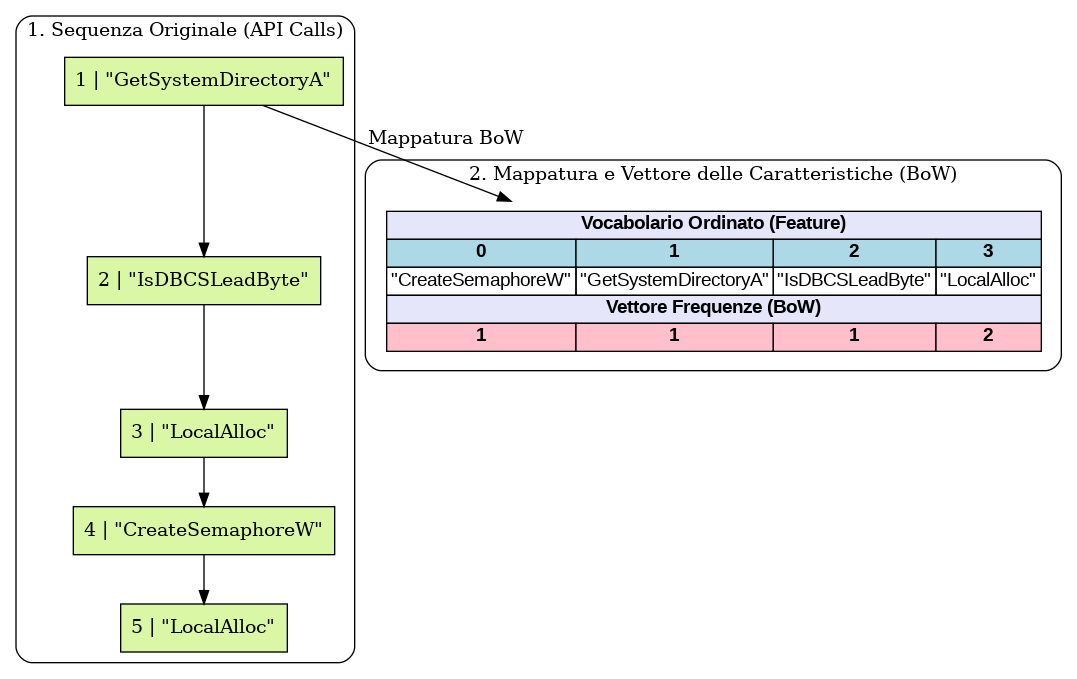
\includegraphics{approccio-proposto/imgs/bow-example.png}%
    }
    \caption{Esempio di ingegnerizzazione delle caratteristiche}
    \label{fig:ign-bow}
\end{figure}

\FloatBarrier

\subsection{Addestramento e Valutazione}

Per ogni dataset e algoritmo di classificazione utilizzato è stato addestrato un modello dedicato.\
L'addestramento dei modelli è stato realizzato tramite molteplici esecuzioni del sistema.\
L'avvio del sistema richiede la specifica dei seguenti parametri di configurazione presenti in \autoref{tab:parametri-config}.

\begin{table}[h!]
    \centering
    \begin{tabular}{lp{10cm}}
        \hline
        \textbf{Parametro}      & \textbf{Descrizione}                                                                                                                                        \\
        \hline
        \texttt{file\_name}     & Nome del file del dataset standardizzato da utilizzare per l’intera fase di addestramento e/o valutazione.                                                  \\[0.5em]
        \texttt{random\_state}  & Valore seme (\textit{seed}) per la gestione dei numeri casuali, utile a garantire la replicabilità delle divisioni del dataset.                             \\[0.5em]
        \texttt{training\_size} & Proporzione del dataset da dedicare al \textit{training set}; la parte complementare è destinata al \textit{testing set}.                                   \\[0.5em]
        \texttt{classifier}     & Algoritmo di classificazione da istanziare e addestrare.                                                                                                    \\[0.5em]
        \texttt{train}          & Flag booleano che forza l’addestramento del modello; se impostato a \texttt{False}, viene riutilizzato un modello precedentemente salvato (se disponibile). \\
        \hline
    \end{tabular}
    \caption{Tabella di configurazione dei parametri del sistema.}
    \label{tab:parametri-config}
\end{table}

\FloatBarrier

Una volta impostati i parametri, il sistema provvede a caricare in memoria il dataset standardizzato corrispondente, applicando la logica descritta in \autoref{sec:ign-bofw} per la rappresentazione
vettoriale delle caratteristiche.
Il dataset così ottenuto viene suddiviso in \textit{training set} e \textit{testing set} secondo la percentuale definita dal parametro \textit{training\_size},
fissato in questo lavoro a $0.8$, corrispondente all'\percc{80} dei dati destinati alla fase di addestramento.\
La divisione è effettuata mediante \textbf{campionamento stratificato}(\textit{Stratified Sampling})\mycite{Wikipedia_campionamento_stratificato},\
in modo da garantire la corretta proporzionalità delle diverse classi di software in entrambi i sottoinsiemi, prevenendo distorsioni\
del modello e assicurando un'adeguata rappresentanza anche delle classi minoritarie.\
Il classificatore sviluppato è di tipo \textbf{supervisionato}, ossia apprende a distinguere le classi a partire da esempi etichettati.
In particolare, il sistema riceve in input il \textit{training set} composto da vettori di caratteristiche e dalle corrispondenti etichette (\textit{goodware}, \textit{dropper},
\textit{trojan}, \dots), e produce in output un modello addestrato capace di associare una classe ai nuovi esempi.
Nel lavoro proposto, il classificatore può essere implementato tramite uno dei due algoritmi considerati: \textit{Random Forest} o \textit{XGBoost},
entrambi forniti dalla libreria \textit{Scikit-learn}\mycite{scikit-learn}.
Una volta completata la \textbf{fase di addestramento}, il modello predice le classi degli esempi nel \textit{testing set} e le confronta con quelle effettive;\
dalla comparazione viene compilata la \textbf{matrice di confusione}.
La \textbf{matrice di confusione} verrà utilizzata per ricavare le metriche di valutazione del modello.